\chapter{Servlets}
Servletler html sayfaları ile java programları arasında bir nevi arayüz olarak tanımlanabilir. Kendileri de birer java programı olan bu kod parçalarının ana amacı MVC (model view controller) yaklaşımı
doğrultusunda iş (business-model) ile web arayüzü arasındaki iletişimi control etmektir. Aslında sadece kontrol değil bizzat kendileri de sayfa generate etmek içinde kullanılabilirler. 

\section{Örnek bir program}
Projemizin dosya düzeni şekil \ref{fig:filetree} de görüldüğü gibidir. Ön alt yapıyı maven ile otomatik de oluşturabiliriz.
\begin{figure}[h]
\centering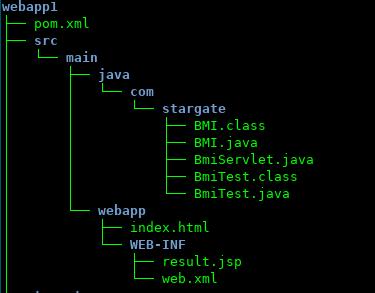
\includegraphics[scale=0.7]{/java/filetree}
\caption{\emph{"webapp1"} Projesinin Dosya Yapısı}
\label{fig:filetree}
\end{figure}
Projeyi derlemek ve hemen kullanıma koymak için maven aracını kullanmak bize büyük esneklik ve kolaylık sağlar. Altta olup bitenden çok kopmadan projenin kontrolü tamamen sizde olur. Özellikle ilk başta bir IDE kullanarak yapılan projeler genellikle ayrıntıya hakim olamama sorununa yol açabilir. 
\subsection{Maven` a Kısa Bir Giriş}%
\label{sub:mavengiris}
C++ için \emph{make} neyse java için textbf{emph{Maven}} odur. Maven aslında  
sadece bir yapılandırma aracı (build tool) değil eklentili yapısı ile tüm projeyi
ve deployment` ı ayarlamaya ve şekillendirmeye yarayan bir araçtır.

Projenin derlenmesi için kaynak (src) klasörünün yanında \emph{pom.xml} adındaki
proje konfigurasyon dosyasının oluşturulması gerekir (Bkz. Şekil \ref{fig:filetree}).

Liste \ref{list:webpom} de pom.xml dosyasının içeriği verilmiştir.
%\begin{lstlisting}
\lstinputlisting[label={list:webpom},caption={Maven Yapılandırma Dosyası: pom.xml},language={XML},breaklines]{/home/cagatay/gitrepo/Ipa-ITBook/konular/java/projects/webProjects/webapp1/pom.xml}
%\end{lstlisting}
